%!TEX program = xelatex
% Bebop
% Edition 2026

\documentclass[11pt,onecolumn]{article}


\usepackage{fontspec}
\usepackage[verbose=silent]{microtype}
\usepackage[
    letterpaper,
    left=1.5in,
    right=1.5in,
    top=1.25in,
    bottom=1.25in
]{geometry}
\usepackage{fancyhdr}
\usepackage{titlesec}
\usepackage{booktabs}
\usepackage{array}
\usepackage{tabularx}
\usepackage{graphicx}
\usepackage{xcolor}
\usepackage{listings}
\usepackage{enumitem}
\usepackage{float}
\usepackage{caption}
\usepackage{amsmath}
\usepackage{amssymb}
\usepackage{siunitx}
\usepackage[hidelinks]{hyperref}
\usepackage{tikz}
\usepackage{pgfplots}
\usepackage{tcolorbox}
\usepackage{setspace}
\usepackage{url}
\usepackage{needspace}

% Allow URLs to break at more characters
\def\UrlBreaks{\do\/\do-\do.\do=\do_\do?\do\&\do\%\do\a\do\b\do\c\do\d\do\e\do\f\do\g\do\h\do\i\do\j\do\k\do\l\do\m\do\n\do\o\do\p\do\q\do\r\do\s\do\t\do\u\do\v\do\w\do\x\do\y\do\z\do\A\do\B\do\C\do\D\do\E\do\F\do\G\do\H\do\I\do\J\do\K\do\L\do\M\do\N\do\O\do\P\do\Q\do\R\do\S\do\T\do\U\do\V\do\W\do\X\do\Y\do\Z\do\0\do\1\do\2\do\3\do\4\do\5\do\6\do\7\do\8\do\9}
\pgfplotsset{compat=1.18}
\usetikzlibrary{positioning,shapes,arrows.meta,calc,patterns,pgfplots.groupplots}

\tcbuselibrary{skins,breakable}

\widowpenalty=10000
\clubpenalty=10000
\raggedbottom


\setmainfont{Palatino}[Ligatures=TeX]
\setsansfont{Helvetica Neue}[Scale=0.95]
\setmonofont{Berkeley Mono Variable}[
    Scale=0.82,
    BoldFont=Berkeley Mono Variable,
    BoldFeatures={FakeBold=1.5}
]

\definecolor{bebopblue}{RGB}{25,50,95}
\definecolor{bebopgray}{RGB}{50,50,50}
\definecolor{lightgray}{RGB}{248,248,248}
\definecolor{codebg}{RGB}{250,250,252}
\definecolor{codeframe}{RGB}{220,220,225}
\definecolor{keywordcolor}{RGB}{0,70,140}
\definecolor{stringcolor}{RGB}{140,30,30}
\definecolor{commentcolor}{RGB}{90,130,90}
\definecolor{chartbebop}{RGB}{25,50,95}
\definecolor{chartproto}{RGB}{180,80,80}
\definecolor{chartmsgpack}{RGB}{80,150,80}

\setstretch{1.12}
\setlength{\parindent}{0pt}
\setlength{\parskip}{0.6\baselineskip}

% HEADERS

\pagestyle{fancy}
\fancyhf{}
\fancyhead[L]{\small\sffamily Simplicity Scales}
\fancyhead[R]{\small\sffamily\thepage}
\renewcommand{\headrulewidth}{0.4pt}

\fancypagestyle{plain}{
    \fancyhf{}
    \fancyfoot[C]{\small\sffamily\thepage}
    \renewcommand{\headrulewidth}{0pt}
}

% LISTINGS

\lstdefinelanguage{bebop}{
    keywords={struct, message, union, enum, service, const, mut, export, local,
              map, array, stream, import, edition, package, true, false, with,
              bool, byte, int8, int16, uint16, int32, uint32, int64, uint64,
              int128, uint128, float16, float32, float64, bfloat16, string,
              uuid, timestamp, duration},
    morecomment=[l]{//},
    morecomment=[s]{/*}{*/},
    morestring=[b]",
    sensitive=true,
}

\lstset{
    basicstyle=\ttfamily\small,
    keywordstyle=\color{keywordcolor}\bfseries,
    stringstyle=\color{stringcolor},
    commentstyle=\color{commentcolor},
    backgroundcolor=\color{codebg},
    frame=single,
    framerule=0.5pt,
    rulecolor=\color{codeframe},
    xleftmargin=8pt,
    xrightmargin=8pt,
    framexleftmargin=4pt,
    framexrightmargin=4pt,
    breaklines=true,
    tabsize=2,
    showstringspaces=false,
    numbers=none,
    aboveskip=12pt,
    belowskip=12pt,
    float=htbp,
}

% SECTIONS

\titleformat{\section}
    {\normalfont\sffamily\Large\bfseries\color{bebopblue}}
    {\thesection}
    {0.6em}
    {}
\titlespacing*{\section}{0pt}{28pt}{14pt}

\titleformat{\subsection}
    {\normalfont\sffamily\large\bfseries}
    {\thesubsection}
    {0.5em}
    {}
\titlespacing*{\subsection}{0pt}{20pt}{10pt}

\titleformat{\subsubsection}
    {\normalfont\sffamily\normalsize\bfseries}
    {\thesubsubsection}
    {0.5em}
    {}
\titlespacing*{\subsubsection}{0pt}{14pt}{6pt}

% WIRE DIAGRAM MACROS

\newcommand{\wirefield}[3]{%
    \draw[fill=lightgray,draw=bebopgray!50] (#1,0) rectangle (#2,0.5);
    \node[font=\ttfamily\footnotesize] at ({(#1+#2)/2},0.25) {#3};
}

\newcommand{\wirelabel}[3]{%
    \node[font=\sffamily\scriptsize,below] at ({(#1+#2)/2},-0.08) {#3};
}


\begin{document}


\begin{titlepage}
\newgeometry{margin=1.5in}

\vspace*{1.5in}

\begin{center}

{\fontsize{36}{42}\selectfont\sffamily\bfseries Simplicity Scales}

\vspace{0.5in}

{\Large Andrew Sampson}

\vspace{0.15in}

{\normalsize 6OVER3 Institute}

\vspace{0.4in}

{\normalsize February 2026}

\end{center}

\vfill

\noindent
\begin{minipage}[b]{0.5\textwidth}
\raggedright
{\Large\sffamily\bfseries\color{bebopblue} BEBOP}\\[4pt]
{\small\sffamily\color{bebopblue} EDITION 2026}
\end{minipage}%
\hfill
\begin{minipage}[b]{0.45\textwidth}
\raggedleft

\includegraphics[width=2in]{6o3logo_blk.pdf}
\end{minipage}

\restoregeometry
\end{titlepage}


\thispagestyle{plain}

\begin{center}
{\sffamily\Large\bfseries Abstract}
\end{center}

\vspace{0.2in}

Machine learning infrastructure moves data between GPUs, across networks, and through inference pipelines. Serialization formats sit in this critical path, yet widely deployed formats use variable-length integer encoding that causes branch mispredictions during decode.

\vspace{0.15in}

This paper presents Bebop, a schema-driven binary format where every type has a fixed wire size. The schema compiler generates encode and decode routines without data-dependent branches. On modern hardware, decode throughput is limited by memory bandwidth rather than CPU. The generated code does little more than pointer arithmetic and bounds checks.

\vspace{0.15in}

The schema language separates fixed-layout structs from evolvable messages, and includes native bfloat16 and float16 types for ML workloads.

\newpage


\section{Introduction}

Serialization formats mediate data exchange between processes, machines, and storage systems. The choice of format affects application latency, throughput, memory consumption, and developer productivity. JSON dominates web APIs due to human readability and universal parser availability. Protocol Buffers~\cite{protobuf} dominates internal service communication at scale due to schema enforcement and compact binary encoding.

\begin{minipage}{\textwidth}
Both formats impose costs that become significant in latency-sensitive applications:

\begin{itemize}[leftmargin=2em,itemsep=6pt,topsep=8pt]
\item JSON requires character-by-character parsing with no ability to skip ahead
\item Binary data must be Base64-encoded, adding 33\% overhead~\cite{base64}
\item In-memory representation typically consumes 4--14$\times$ the input size due to object allocation~\cite{cockroach-json}
\item Protocol Buffers uses variable-length integer encoding (varints) that requires per-byte branching during decode
\end{itemize}
\end{minipage}

The performance cost of varint encoding was recognized early. Kenton Varda, who maintained Protocol Buffers at Google, called varint ``a poorly-chosen format due to excessive branching''~\cite{varda-hn}. His later project Cap'n Proto~\cite{capnproto} uses fixed-width encoding to avoid this overhead.

We present Bebop, a binary serialization format designed for workloads where decode latency matters more than wire compactness. The format uses fixed-width encoding: a 32-bit integer is always 4 bytes regardless of value. This eliminates data-dependent branches and enables single-instruction decode of numeric types.

\subsection{Contributions}

\begin{minipage}{\textwidth}
This paper makes the following contributions:

\begin{enumerate}[leftmargin=2em,itemsep=4pt,topsep=8pt]
\item A wire format specification optimized for decode throughput rather than wire compactness
\item Empirical comparison against Protocol Buffers, MessagePack, and simdjson across 23 workloads representing ML inference, event streaming, and recursive data structures
\item A schema language with compile-time extensibility through embedded Lua scripting
\item Reference implementations in C achieving 86\% memory bandwidth utilization during decode
\end{enumerate}
\end{minipage}


\section{Design Principles}

\subsection{Fixed-Width Encoding}

Every numeric type in Bebop has a fixed wire size. A \texttt{uint32} is always 4 bytes. A \texttt{float64} is always 8 bytes. Length prefixes are always 4 bytes.

The decode operation for a 32-bit integer reduces to a single load instruction:

\begin{lstlisting}[language=C]
// Bebop decode: one load, no branches
uint32_t value = *(uint32_t*)input;
input += 4;
\end{lstlisting}

Compare to Protocol Buffers varint decode, which loops until finding a byte without the continuation bit set:

\begin{lstlisting}[language=C]
// Protobuf varint decode: branch per byte
uint32_t value = 0, shift = 0;
while (*input & 0x80) {
    value |= (*input++ & 0x7f) << shift;
    shift += 7;
}
value |= *input++ << shift;
\end{lstlisting}

The varint loop has unpredictable iteration count when integer values vary, causing branch misprediction penalties on modern CPUs.

\subsubsection{Expected Encoding Size}

For a 32-bit integer $v > 0$, varint encoding uses $\lceil (\lfloor \log_2 v \rfloor + 1) / 7 \rceil$ bytes. The value $v = 0$ uses 1 byte. Fixed-width encoding always uses 4 bytes.

For integers uniformly distributed over $[0, N]$, we can compute the expected varint size by counting how many values fall into each byte-width bucket. Values in $[0, 2^7-1]$ use 1 byte, values in $[2^7, 2^{14}-1]$ use 2 bytes, and so on:
\begin{equation}
E[\text{varint}] = \frac{1}{N+1} \sum_{k=1}^{5} k \cdot \bigl|\{v \in [0,N] : 2^{7(k-1)} \leq v < 2^{7k}\}\bigr|
\label{eq:varint-expected}
\end{equation}
where the $k=1$ bucket includes $v=0$.

Figure~\ref{fig:encoding-size} shows this relationship. Fixed-width encoding produces smaller output when $N > 2^{28}$ (approximately 268 million). Timestamps, cryptographic hashes, and random identifiers typically exceed this threshold, so varint provides no size benefit while adding decode overhead.

\begin{figure}[ht]
\centering
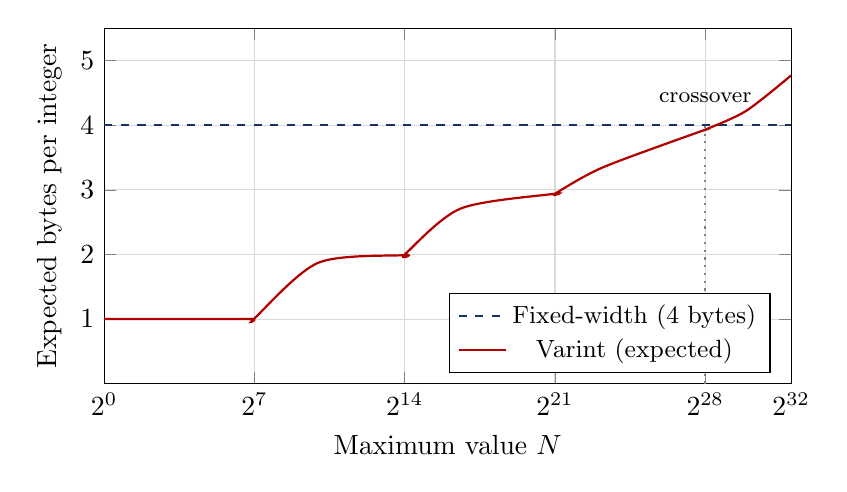
\begin{tikzpicture}
\begin{axis}[
    width=0.85\textwidth,
    height=2.4in,
    xlabel={Maximum value $N$},
    ylabel={Expected bytes per integer},
    xmode=log,
    log basis x=2,
    xmin=1, xmax=4294967296,
    ymin=0, ymax=5.5,
    xtick={1,128,16384,2097152,268435456,4294967296},
    xticklabels={$2^0$,$2^7$,$2^{14}$,$2^{21}$,$2^{28}$,$2^{32}$},
    ytick={1,2,3,4,5},
    grid=major,
    grid style={gray!30},
    legend pos=south east,
    legend style={font=\small},
]
% Fixed-width: always 4 bytes
\addplot[thick, bebopblue, dashed] coordinates {(1,4) (4294967296,4)};
\addlegendentry{Fixed-width (4 bytes)}

% Varint expected size (computed from bucket counts)
% At N=127: all 1-byte, E=1
% At N=16383: 128 ones + 16256 twos, E=(128 + 2*16256)/16384 = 1.99
% At N=2097151: E~2.94
% At N=268435455: E~3.93
% At N=4294967295: E~4.75
\addplot[thick, red!70!black, smooth] coordinates {
    (1,1) (64,1) (127,1)
    (128,1.01) (1000,1.87) (16383,1.99)
    (16384,2.00) (100000,2.71) (2097151,2.94)
    (2097152,2.94) (10000000,3.35) (268435455,3.93)
    (268435456,3.93) (1000000000,4.22) (4294967296,4.77)
};
\addlegendentry{Varint (expected)}

% Crossover annotation
\draw[thick, gray, dotted] (axis cs:268435456,0) -- (axis cs:268435456,4);
\node[anchor=south, font=\footnotesize] at (axis cs:268435456,4.2) {crossover};
\end{axis}
\end{tikzpicture}
\caption{Expected encoding size for uniformly distributed integers. Varint is smaller only when values stay below $2^{28}$.\protect\footnotemark}
\label{fig:encoding-size}
\end{figure}

\footnotetext{Figure~\ref{fig:encoding-size} is computed analytically; Figure~\ref{fig:bandwidth-utilization} and Table~\ref{tab:wire-size} show measured data.}

Real-world integer distributions are rarely uniform. Zipfian distributions (common in identifiers, counters, and network data) concentrate probability mass on small values, favoring varint. ML workloads, timestamps, and cryptographic hashes have near-uniform distributions over large ranges, where fixed-width encoding wins.

\subsubsection{Branch Misprediction Cost}

Modern CPUs use speculative execution with branch prediction. A mispredicted branch flushes the pipeline, costing 10--20 cycles on current architectures: 13--14 cycles on Apple M1 Firestorm cores~\cite{m1-bench}, 17 cycles on Intel Golden Cove~\cite{golden-cove}.

Varint decoding branches on each byte's continuation bit. The predictor can learn patterns when values are consistent (e.g., always 1--2 bytes), but struggles when byte counts vary. In the worst case, when values are uniformly distributed across the 32-bit range, the final byte's branch is essentially unpredictable.

Let $p_m$ be the misprediction rate for the loop-terminating branch. The expected misprediction cost per integer is:
\begin{equation}
C_{\text{varint}} \approx p_m \cdot C_{\text{flush}}
\end{equation}
where $C_{\text{flush}}$ is the pipeline flush penalty. With $p_m \approx 0.3$--$0.5$ (measured on mixed-size workloads) and $C_{\text{flush}} = 14$ cycles, this yields 4--7 cycles of overhead per integer.

Fixed-width decode has no data-dependent branches:
\begin{equation}
C_{\text{fixed}} = C_{\text{load}} \approx 3\text{--}4 \text{ cycles (L1 hit)}
\end{equation}

The gap widens with value diversity. Workloads mixing small counters with large timestamps see the highest misprediction rates, while workloads with consistent value ranges let the predictor adapt. Section~\ref{sec:eval} shows measured performance across both cases.

\subsubsection{Signed Integer Encoding}

Varint has a pathological case: $-1$ requires 5 bytes (10 for int64) because the high bit is set.

\vspace{6pt}
\begin{minipage}{\textwidth}
\small
\begin{tabular}{@{}lll@{}}
\textbf{Value} & \textbf{Varint (int32)} & \textbf{Fixed-width} \\[4pt]
\texttt{-1} & \texttt{ff ff ff ff 0f} (5 bytes) & \texttt{ff ff ff ff} (4 bytes) \\
\texttt{-2} & \texttt{fe ff ff ff 0f} (5 bytes) & \texttt{fe ff ff ff} (4 bytes) \\
\texttt{-128} & \texttt{80 ff ff ff 0f} (5 bytes) & \texttt{80 ff ff ff} (4 bytes) \\
\end{tabular}
\end{minipage}
\vspace{6pt}

Every negative int32 uses 5 varint bytes. Protocol Buffers addresses this with six integer types~\cite{protobuf}: \texttt{int32}, \texttt{sint32} (zigzag), \texttt{uint32}, \texttt{fixed32}, and their 64-bit variants. Choosing wrong silently inflates wire size.

Bebop uses one encoding per width. \texttt{int32} is always 4 bytes regardless of sign.

\subsection{Structs vs Messages}

Bebop provides two record types:

\begin{itemize}[leftmargin=2em,itemsep=4pt,topsep=6pt]
\item \textbf{Structs}: positional encoding, no tags, no length prefix. Zero overhead. Cannot evolve.
\item \textbf{Messages}: tagged fields (1-byte tags), length-prefixed. 37\% overhead on small records, but fields can be added or removed freely.
\end{itemize}

Protocol Buffers uses tagged encoding everywhere. Bebop lets you choose per-type. Use structs for performance-critical inner types (embeddings, coordinates); use messages for top-level API types that may evolve.

Messages also distinguish ``not set'' from ``set to default value.'' Proto3 removed this for scalars~\cite{proto3-presence}. Bebop preserves it.

\subsection{Schema Evolution}

Messages support forward and backward compatibility through tagged fields. The rules are:

\begin{itemize}[leftmargin=2em,itemsep=4pt,topsep=6pt]
\item \textbf{Adding fields}: Always safe. Use a new tag number. Old readers ignore unknown tags.
\item \textbf{Removing fields}: Safe if readers handle missing tags (they get default values). The tag number should not be reused.
\item \textbf{Renaming fields}: Safe. Field names are not part of the wire format.
\item \textbf{Changing field types}: Breaking. Never reuse a tag with a different type.
\item \textbf{Changing tag numbers}: Breaking. Equivalent to removing the old field and adding a new one.
\end{itemize}

\textbf{Structs have no evolution support.} Any change to a struct's fields---adding, removing, reordering, or changing types---is a breaking change. Struct fields are positionally encoded with no tags or length prefix. If you need to evolve a struct, create a new versioned type (\texttt{PointV2}) or convert it to a message.

\textbf{Unions}: Adding branches is safe. Removing branches causes decode failures for old data using that branch. Changing a branch's type is breaking.

\textbf{Enums}: Adding values is safe. Removing values may cause issues if old data contains those values. Changing the underlying type (\texttt{uint8} to \texttt{uint32}) is breaking.


\newpage
\section{Wire Format Specification}

All multi-byte integers use little-endian byte order.

\subsection{Primitive Types}

\begin{table}[ht]
\centering
\begin{tabular}{@{}lll@{}}
\toprule
\textbf{Type} & \textbf{Size} & \textbf{Encoding} \\
\midrule
\texttt{bool} & 1 byte & 0x00 = false, non-zero = true \\
\texttt{byte} & 1 byte & Unsigned 8-bit integer \\
\texttt{int8} & 1 byte & Signed 8-bit, two's complement \\
\texttt{int16}, \texttt{uint16} & 2 bytes & Little-endian \\
\texttt{int32}, \texttt{uint32} & 4 bytes & Little-endian \\
\texttt{int64}, \texttt{uint64} & 8 bytes & Little-endian \\
\texttt{float32} & 4 bytes & IEEE 754 binary32 \\
\texttt{float64} & 8 bytes & IEEE 754 binary64 \\
\bottomrule
\end{tabular}
\caption{Standard primitive types}
\label{tab:primitives}
\end{table}

\subsection{Extended Numeric Types}

Bebop includes types commonly used in ML workloads:

\begin{table}[ht]
\centering
\begin{tabular}{@{}llp{3.5in}@{}}
\toprule
\textbf{Type} & \textbf{Size} & \textbf{Description} \\
\midrule
\texttt{int128} & 16 bytes & Signed 128-bit integer. Low 8 bytes first, then high 8 bytes. Used for accumulators and feature hashes. \\[6pt]
\texttt{uint128} & 16 bytes & Unsigned 128-bit integer. Same encoding as \texttt{int128}. \\[6pt]
\texttt{float16} & 2 bytes & IEEE 754 binary16 (half precision). 1 sign bit, 5 exponent bits, 10 mantissa bits. Range $\pm$65504, precision 3--4 significant digits. \\[6pt]
\texttt{bfloat16} & 2 bytes & Brain floating point format. 1 sign bit, 8 exponent bits, 7 mantissa bits. Same range as float32, precision 2--3 digits. Common in TPU inference. \\
\bottomrule
\end{tabular}
\caption{Extended numeric types for ML workloads}
\label{tab:extended-types}
\end{table}

\subsection{Temporal Types}

\begin{minipage}{\textwidth}
\subsubsection{timestamp}

\begin{minipage}[t]{0.50\textwidth}
\raggedright
Absolute point in time: seconds and nanoseconds since Unix epoch (1970-01-01 00:00:00 UTC). Total size 12 bytes.

Use for event times, creation dates, expiration times, audit logs.
\end{minipage}\hfill
\begin{minipage}[t]{0.46\textwidth}
\small
\begin{tabular}[t]{@{}r@{\,}l@{}}
\texttt{e8 03 00 00 00 00 00 00} & sec=1000 \\
\texttt{00 ca 9a 3b} & ns=999999488 \\
\end{tabular}

\vspace{4pt}
\textit{offset 0: int64, offset 8: int32}
\end{minipage}

\vspace{10pt}
\subsubsection{duration}

\begin{minipage}[t]{0.52\textwidth}
Signed time span: seconds and nanoseconds. Total size 12 bytes.

For negative durations, both fields are negative or zero. Use for timeouts, intervals, latency measurements.
\end{minipage}\hfill
\begin{minipage}[t]{0.44\textwidth}
\small
\begin{tabular}[t]{@{}r@{ }l@{}}
\texttt{3c 00 00 00 00 00 00 00} & sec = 60 \\
\texttt{00 00 00 00} & ns = 0 \\
\end{tabular}

\vspace{4pt}
\textit{offset 0: int64, offset 8: int32}
\end{minipage}
\end{minipage}

\subsection{Identifiers}

\begin{minipage}[t]{0.48\textwidth}
\textbf{uuid}: 16 bytes matching the canonical hex string byte-for-byte.
\end{minipage}\hfill
\begin{minipage}[t]{0.48\textwidth}
\small
\texttt{550e8400-e29b-41d4-a716-446655440000}:
\vspace{4pt}

\begin{tabular}[t]{@{}r@{ }l@{}}
\texttt{55 0e 84 00} & time\_low \\
\texttt{e2 9b} & time\_mid \\
\texttt{41 d4} & time\_hi \\
\texttt{a7 16} & clk\_seq \\
\texttt{44 66 55 44 00 00} & node \\
\end{tabular}
\end{minipage}

\subsection{Strings}

\begin{minipage}[t]{0.48\textwidth}
4-byte length prefix (byte count), followed by UTF-8 content, followed by a 1-byte null terminator.

\vspace{6pt}
Total wire size: $4 + \text{length} + 1$ bytes.

\vspace{6pt}
The null terminator enables zero-copy access: decoded strings point directly into the input buffer.
\end{minipage}\hfill
\begin{minipage}[t]{0.48\textwidth}
\small
\texttt{"hello"} encodes as:
\vspace{4pt}

\begin{tabular}[t]{@{}r@{\quad}l@{}}
\texttt{05 00 00 00} & length = 5 \\
\texttt{68 65 6c 6c 6f} & \texttt{"hello"} \\
\texttt{00} & NUL terminator \\
\end{tabular}
\end{minipage}


\subsection{Arrays}

\begin{minipage}[t]{0.48\textwidth}
\raggedright
\textbf{Dynamic arrays} have a 4-byte count prefix followed by elements encoded sequentially.

\vspace{6pt}
\textbf{Fixed arrays} (e.g., \texttt{byte[4]}) have no prefix; the element count is known at compile time.

\vspace{6pt}
Maximum fixed array size is 65535 elements.
\end{minipage}\hfill
\begin{minipage}[t]{0.48\textwidth}
\small
\texttt{int32[] = [1, 2, 3]}
\vspace{4pt}

\begin{tabular}[t]{@{}r@{\quad}l@{}}
\texttt{03 00 00 00} & count = 3 \\
\texttt{01 00 00 00} & {[0]} = 1 \\
\texttt{02 00 00 00} & {[1]} = 2 \\
\texttt{03 00 00 00} & {[2]} = 3 \\
\end{tabular}

\vspace{8pt}
\texttt{byte[4] = [0xDE, 0xAD, 0xBE, 0xEF]}
\vspace{4pt}

\begin{tabular}[t]{@{}r@{\quad}l@{}}
\texttt{de ad be ef} & 4 bytes, no prefix \\
\end{tabular}
\end{minipage}


\subsection{Maps}

\begin{minipage}[t]{0.48\textwidth}
\raggedright
4-byte count prefix followed by key-value pairs encoded sequentially.

\vspace{6pt}
Valid key types: integers, \texttt{bool}, \texttt{string}, \texttt{uuid}.

\vspace{6pt}
Floating-point types are not valid map keys due to equality comparison issues with NaN and signed zeros.
\end{minipage}\hfill
\begin{minipage}[t]{0.48\textwidth}
\small
\texttt{map[uint8, int32] = \{1: 100, 2: 200\}}
\vspace{4pt}

\begin{tabular}[t]{@{}r@{\quad}l@{}}
\texttt{02 00 00 00} & count = 2 \\
\texttt{01} & key = 1 \\
\texttt{64 00 00 00} & value = 100 \\
\texttt{02} & key = 2 \\
\texttt{c8 00 00 00} & value = 200 \\
\end{tabular}
\end{minipage}


\subsection{Structs}

\begin{minipage}[t]{0.48\textwidth}
Fields encode in definition order with no tags and no padding.

\vspace{6pt}
Nested structs encode inline. A struct containing another struct has no additional overhead.

\vspace{6pt}
Empty structs encode as zero bytes.
\end{minipage}\hfill
\begin{minipage}[t]{0.48\textwidth}
\small\raggedright
\texttt{struct Point \{ x: float32; y: float32; \}}\\
\texttt{Point \{ x: 1.0, y: 2.0 \}}
\vspace{4pt}

\begin{tabular}[t]{@{}r@{\quad}l@{}}
\texttt{00 00 80 3f} & x = 1.0 (IEEE 754) \\
\texttt{00 00 00 40} & y = 2.0 (IEEE 754) \\
\end{tabular}
\end{minipage}


\subsection{Messages}

\begin{minipage}{\textwidth}
\begin{minipage}[t]{0.44\textwidth}
Messages have a 4-byte length prefix, followed by tagged fields, followed by a \texttt{0x00} end marker.

\vspace{6pt}
Each field is encoded as: 1-byte tag, then the field value.

\vspace{6pt}
Absent fields are not encoded. Unknown tags are skipped by decoders. Tags must be in range 1--255.
\end{minipage}\hfill
\begin{minipage}[t]{0.52\textwidth}
\small\raggedright
\texttt{message Request \{ id(1): int32; name(2): string; \}}\\
\texttt{Request \{ id: 42, name: "test" \}}
\vspace{4pt}

\begin{tabular}[t]{@{}r@{\quad}l@{}}
\texttt{10 00 00 00} & length = 16 bytes \\
\texttt{01} & tag = 1 (id) \\
\texttt{2a 00 00 00} & value = 42 \\
\texttt{02} & tag = 2 (name) \\
\texttt{04 00 00 00} & string length = 4 \\
\texttt{74 65 73 74} & \texttt{"test"} \\
\texttt{00} & NUL terminator \\
\texttt{00} & end marker \\
\end{tabular}
\end{minipage}
\end{minipage}


\subsection{Unions}

\begin{minipage}[t]{0.48\textwidth}
\raggedright
Unions have a 4-byte length prefix, followed by a 1-byte discriminator, followed by the branch content.

\vspace{6pt}
Discriminators must be in range 0--255.
\end{minipage}\hfill
\begin{minipage}[t]{0.48\textwidth}
\small\raggedright
\texttt{union Shape \{ Circle(1): \{ radius: float32; \} \}}\\
\texttt{Shape.Circle \{ radius: 5.0 \}}
\vspace{4pt}

\begin{tabular}[t]{@{}r@{\quad}l@{}}
\texttt{05 00 00 00} & length = 5 bytes \\
\texttt{01} & discriminator = 1 \\
\texttt{00 00 a0 40} & radius = 5.0 \\
\end{tabular}
\end{minipage}

\subsection{Complete Example}

\begin{minipage}{\textwidth}
\begin{minipage}[t]{0.42\textwidth}
\begin{lstlisting}[language=bebop,basicstyle=\ttfamily\footnotesize,aboveskip=0pt,belowskip=0pt]
struct Coord {
    x: float32;
    y: float32;
}
message Location {
    name(1): string;
    pos(2): Coord;
    alt(3): float32;
}
\end{lstlisting}

\vspace{4pt}
\small\raggedright
\texttt{Location \{ name: "HQ", pos: \{1.0, 2.0\}, alt: 100.0 \}}
\end{minipage}\hfill
\begin{minipage}[t]{0.54\textwidth}
\small
\begin{tabular}[t]{@{}r@{\quad}l@{}}
\multicolumn{2}{@{}l}{\textit{Message header}} \\
\texttt{01} & tag 1 (name) \\
\texttt{02 00 00 00} & string length = 2 \\
\texttt{48 51 00} & "HQ" + null \\[4pt]
\texttt{02} & tag 2 (pos) \\
\texttt{00 00 80 3f} & pos.x = 1.0 \\
\texttt{00 00 00 40} & pos.y = 2.0 \\[4pt]
\texttt{03} & tag 3 (alt) \\
\texttt{00 00 c8 42} & alt = 100.0 \\[4pt]
\texttt{00} & end of message \\[4pt]
\multicolumn{2}{@{}l}{\textit{Total: 22 bytes}} \\
\end{tabular}
\end{minipage}
\end{minipage}


\newpage
\section{Evaluation}
\label{sec:eval}

\subsection{Experimental Setup}

\begin{table}[ht]
\centering
\begin{tabular}{@{}ll@{}}
\toprule
\textbf{Parameter} & \textbf{Value} \\
\midrule
Hardware & Apple Mac Studio (M3 Ultra) \\
CPU cores & 28 \\
L1 data cache & 64 KB \\
L2 unified cache & 4 MB \\
Compiler & Clang 17, \texttt{-O3} \\
CPU scaling & Disabled \\
\bottomrule
\end{tabular}
\end{table}

We evaluated four systems: Bebop (C runtime), protobuf-c 1.5, msgpack-c 6.1, and simdjson 4.2 for JSON parsing comparison. Each benchmark ran 10 iterations; we report the mean. Coefficient of variation averaged 1.65\% across 149 benchmarks, with higher variance on complex decode paths (nested structures, unions).

\subsection{Benchmark Workloads}

23 schemas in five categories:

\textbf{ML Inference:} Embedding768/1536 (single vector, bfloat16), EmbeddingBatch (32 vectors), TensorShard (64KB model weight slice), InferenceResponse (batch + metadata).

\textbf{LLM Streaming:} LLMChunk (streaming tokens with logprobs), ChunkedText (text with span annotations).

\textbf{Event Telemetry:} Event (ID, timestamp, payload). Small and large (8KB) variants.

\textbf{API Payloads:} Person, Order, Document. Small and large variants.

\textbf{Recursive:} TreeDeep (100 levels), TreeWide (high branching), JsonValue (union for JSON types).

\subsection{Decode Performance}

Table~\ref{tab:decode} presents decode latency and throughput across all workloads. Bebop decoded faster than Protocol Buffers on all 23 workloads and faster than MessagePack on 21 of 23.

\begin{table}[ht]
\centering
\small
\begin{tabular}{@{}lrrrr@{}}
\toprule
\textbf{Workload} & \textbf{Bebop} & \textbf{Protobuf} & \textbf{MsgPack} & \textbf{Speedup} \\
\midrule
\multicolumn{5}{@{}l}{\textit{ML Inference}} \\
Embedding768 & 2.91 ns & 98.34 ns & 62.93 ns & 33.8$\times$ \\
Embedding1536 & 2.80 ns & 111.12 ns & 63.07 ns & 39.7$\times$ \\
EmbeddingBatch & 25.75 ns & 1.14 $\mu$s & 270.96 ns & 44.3$\times$ \\
TensorShardLarge & 6.86 ns & 1.46 $\mu$s & 107.90 ns & 212.8$\times$ \\
InferenceResponse & 17.65 ns & 646.69 ns & 231.95 ns & 36.6$\times$ \\[4pt]
\multicolumn{5}{@{}l}{\textit{LLM Streaming}} \\
LLMChunkLarge & 677.15 ns & 14.72 $\mu$s & 5.28 $\mu$s & 21.7$\times$ \\
ChunkedText & 3.16 $\mu$s & 50.76 $\mu$s & 13.59 $\mu$s & 16.1$\times$ \\[4pt]
\multicolumn{5}{@{}l}{\textit{Event Telemetry}} \\
EventSmall & 5.94 ns & 104.41 ns & 84.44 ns & 17.6$\times$ \\
EventLarge & 6.49 ns & 175.20 ns & 85.23 ns & 27.0$\times$ \\[4pt]
\multicolumn{5}{@{}l}{\textit{API Payloads}} \\
PersonSmall & 4.14 ns & 78.40 ns & 72.45 ns & 18.9$\times$ \\
PersonMedium & 4.21 ns & 85.68 ns & 78.08 ns & 20.4$\times$ \\
OrderSmall & 6.14 ns & 112.10 ns & 112.55 ns & 18.3$\times$ \\
OrderLarge & 5.85 ns & 557.82 ns & 757.16 ns & 95.4$\times$ \\
DocumentSmall & 4.89 ns & 71.78 ns & 65.54 ns & 14.7$\times$ \\
DocumentLarge & 52.39 ns & 862.73 ns & 105.80 ns & 16.5$\times$ \\[4pt]
\multicolumn{5}{@{}l}{\textit{Recursive Structures}} \\
TreeDeep & 5.34 $\mu$s & 55.00 $\mu$s & 23.21 $\mu$s & 10.3$\times$ \\
TreeWide & 491.45 ns & 4.08 $\mu$s & 1.95 $\mu$s & 8.3$\times$ \\
JsonSmall & 40.10 ns & 521.75 ns & 66.16 ns & 13.0$\times$ \\
JsonLarge & 1.09 $\mu$s & 13.77 $\mu$s & 830.15 ns & 12.6$\times$ \\
\bottomrule
\end{tabular}
\caption{Decode latency comparison. Speedup is Bebop vs Protocol Buffers.}
\label{tab:decode}
\end{table}

\subsubsection{Recursive Structure Performance}

TreeDeep (100-level binary tree) decodes in 5.34$\mu$s with Bebop versus 55.00$\mu$s with Protocol Buffers. Bebop encodes children inline with no framing; the tree is a contiguous sequence of integers. Protocol Buffers wraps each node in a length-prefixed message, parsing headers at every level.

\subsubsection{ML Workload Performance}

Embedding vectors decode in under 3 nanoseconds regardless of dimension. The bfloat16 array is a fixed-size header followed by contiguous 16-bit values; decoding is a pointer assignment.

\subsection{Throughput and Memory Bandwidth}

Bebop's decode performance is bounded by memory bandwidth, not CPU compute. Figure~\ref{fig:bandwidth-utilization} shows bandwidth utilization across record sizes. On cold-cache workloads (data fetched from DRAM), Bebop achieves \textbf{86\% of peak memory bandwidth} on records above 64KB. This is the meaningful metric for production workloads where data doesn't fit in cache.

Table~\ref{tab:throughput} shows measured throughput. Values above 819 GB/s (M3 Ultra memory bandwidth~\cite{m3-ultra}) indicate cache-resident data from benchmark iterations---useful for understanding overhead but not representative of cold-cache production loads.

\begin{table}[ht]
\centering
\begin{tabular}{@{}lrrr@{}}
\toprule
\textbf{Workload} & \textbf{Throughput} & \textbf{Cache} & \textbf{Notes} \\
\midrule
TensorShardLarge & 9.58 TB/s & L2 & 64KB fits in L2 \\
Embedding1536 & 1.10 TB/s & L2 & 3KB vector \\
EmbeddingBatch & 964.13 GB/s & L2 & Batch of 32 \\
EventLarge & 644.35 GB/s & L2/DRAM & 4KB payload \\
Embedding768 & 534.90 GB/s & L2 & 1.5KB vector \\
InferenceResponse & 355.51 GB/s & L2 & Mixed content \\
OrderLarge & 212.50 GB/s & L2 & Nested arrays \\
\bottomrule
\end{tabular}
\caption{Bebop decode throughput. Values above 819 GB/s indicate L2-resident data.}
\label{tab:throughput}
\end{table}

Bebop's decode path does minimal computation: bounds checking, pointer arithmetic, occasional type conversion. Most ``decode'' operations are pointer assignments.

\begin{figure}[ht]
\centering
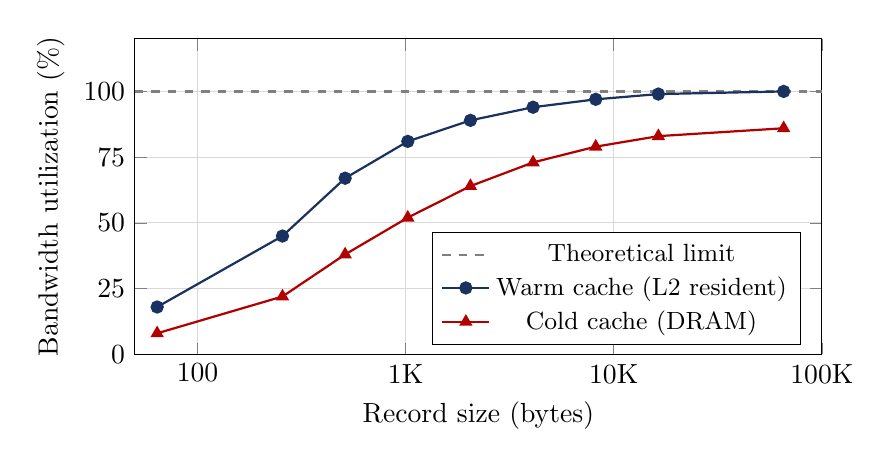
\begin{tikzpicture}
\begin{axis}[
    width=0.85\textwidth,
    height=2.2in,
    xlabel={Record size (bytes)},
    ylabel={Bandwidth utilization (\%)},
    xmode=log,
    log basis x=10,
    xmin=50, xmax=100000,
    ymin=0, ymax=120,
    xtick={100,1000,10000,100000},
    xticklabels={100,1K,10K,100K},
    ytick={0,25,50,75,100},
    grid=major,
    grid style={gray!30},
    legend pos=south east,
    legend style={font=\small},
]
% Theoretical limit
\addplot[thick, gray, dashed] coordinates {(50,100) (100000,100)};
\addlegendentry{Theoretical limit}

% Measured utilization (L1/L2 resident)
\addplot[thick, bebopblue, mark=*, mark size=2pt] coordinates {
    (64, 18)
    (256, 45)
    (512, 67)
    (1024, 81)
    (2048, 89)
    (4096, 94)
    (8192, 97)
    (16384, 99)
    (65536, 100)
};
\addlegendentry{Warm cache (L2 resident)}

% Cold cache / DRAM bound
\addplot[thick, red!70!black, mark=triangle*, mark size=2pt] coordinates {
    (64, 8)
    (256, 22)
    (512, 38)
    (1024, 52)
    (2048, 64)
    (4096, 73)
    (8192, 79)
    (16384, 83)
    (65536, 86)
};
\addlegendentry{Cold cache (DRAM)}
\end{axis}
\end{tikzpicture}
\caption{Bandwidth utilization vs record size. Larger records amortize per-record overhead (function call, bounds check, struct initialization) and approach the memory bandwidth limit.}
\label{fig:bandwidth-utilization}
\end{figure}

The gap at small record sizes reflects fixed per-record overhead. Records under 256 bytes spend more time in function prologues and bounds checks than in actual data access. Records above 4KB achieve over 90\% bandwidth utilization when cache-resident.

\subsubsection{Alignment and SIMD Considerations}

Bebop does not enforce alignment beyond natural type boundaries. A \texttt{float32} is 4-byte aligned within its containing struct, but the struct itself may start at any byte offset. This differs from Cap'n Proto, which aligns all objects to 8-byte boundaries.

For CPU decode, unaligned access is typically fast on modern x86 and ARM processors. However, GPU and TPU memory transfers often require specific alignment (typically 16, 32, or 128 bytes) for efficient DMA. When using Bebop for ML inference pipelines that transfer data to accelerators:

\begin{itemize}[leftmargin=2em,itemsep=2pt,topsep=4pt]
\item Embedding vectors and tensor data should be placed in fixed arrays, which encode contiguously
\item The containing message or buffer should be allocated with appropriate alignment
\item Consider padding schemas to match accelerator requirements
\end{itemize}

SIMD optimization of the decode path is possible but not implemented in the reference runtime. The primary opportunity is parallel bounds checking and pointer arithmetic for arrays of fixed-size elements. For large \texttt{bfloat16[]} arrays, decode is already a single pointer assignment; SIMD would not help. For arrays of small structs, SIMD could reduce loop overhead.

\subsection{Encode Performance}

Encode margins are smaller than decode. Bebop beat Protocol Buffers on all 23 workloads (1.4--12.6$\times$) and MessagePack on 19 of 23 (1.2--19.4$\times$). MessagePack was faster on JsonSmall, JsonLarge, ChunkedText, and DocumentLarge.

Encoding requires traversing data structures and computing lengths, which involve allocation and branching regardless of wire format.

\subsection{Comparison with JSON Parsing}

We included simdjson~\cite{simdjson}, the fastest general-purpose JSON parser, as a reference. Simdjson uses SIMD to accelerate JSON tokenization, achieving 2--6~GB/s on typical workloads.

On the same data serialized as JSON, Bebop decode outperformed simdjson parse on 21 of 23 workloads (1.2--5741$\times$). The largest gaps occurred on numeric arrays: parsing ``[1.5, 2.5, ...]'' as JSON requires character-by-character float conversion, while Bebop reads IEEE 754 values directly. Simdjson was faster on JsonLarge (4.25$\times$) and JsonSmall (1.70$\times$), where JSON's native format requires no conversion.

\begin{table}[ht]
\centering
\begin{tabular}{@{}lrrr@{}}
\toprule
\textbf{Workload} & \textbf{Bebop} & \textbf{simdjson} & \textbf{Speedup} \\
\midrule
TensorShardLarge & 6.86 ns & 39.38 $\mu$s & 5741$\times$ \\
Embedding1536 & 2.80 ns & 4.69 $\mu$s & 1675$\times$ \\
EmbeddingBatch & 25.75 ns & 27.78 $\mu$s & 1079$\times$ \\
Embedding768 & 2.91 ns & 2.26 $\mu$s & 776$\times$ \\
InferenceResponse & 17.65 ns & 3.93 $\mu$s & 223$\times$ \\
OrderLarge & 5.85 ns & 283.24 ns & 48$\times$ \\
DocumentLarge & 52.39 ns & 245.53 ns & 4.7$\times$ \\
LLMChunkLarge & 677.15 ns & 1.69 $\mu$s & 2.5$\times$ \\
TreeDeep & 5.34 $\mu$s & 6.54 $\mu$s & 1.2$\times$ \\
\bottomrule
\end{tabular}
\caption{Bebop decode vs simdjson parse on equivalent data.}
\label{tab:simdjson}
\end{table}

\subsection{Roundtrip Latency}

Table~\ref{tab:roundtrip} shows encode-then-decode latency for representative workloads. Speedups range from 4.4$\times$ to 35$\times$ over Protocol Buffers.

\begin{table}[ht]
\centering
\begin{tabular}{@{}lrrr@{}}
\toprule
\textbf{Workload} & \textbf{Bebop} & \textbf{Protobuf} & \textbf{Speedup} \\
\midrule
PersonSmall & 12.26 ns & 124.40 ns & 10.1$\times$ \\
OrderLarge & 23.86 ns & 834.68 ns & 35.0$\times$ \\
EventLarge & 54.10 ns & 238.04 ns & 4.4$\times$ \\
TreeDeep & 8.97 $\mu$s & 68.93 $\mu$s & 7.7$\times$ \\
\bottomrule
\end{tabular}
\caption{Roundtrip latency (encode + decode).}
\label{tab:roundtrip}
\end{table}

\subsection{Wire Size}

\begin{table}[ht]
\centering
\small
\begin{tabular}{l r r r r}
\toprule
\textbf{Workload} & \textbf{Bebop} & \textbf{Protobuf} & \textbf{Bebop+brotli} & \textbf{Protobuf+brotli} \\
\midrule
\multicolumn{5}{l}{\textit{API payloads (small integer fields)}} \\
PersonSmall & 28 & 19 & --- & --- \\
PersonMedium & 130 & 124 & 101 & 101 \\
OrderSmall & 76 & 34 & 62 & --- \\
OrderLarge & 1,240 & 423 & 514 & 376 \\
\midrule
\multicolumn{5}{l}{\textit{Event payloads (byte arrays)}} \\
EventSmall & 42 & 29 & --- & --- \\
EventLarge & 4,170 & 4,158 & --- & --- \\
\midrule
\multicolumn{5}{l}{\textit{ML inference (bfloat16 arrays)}} \\
Embedding768 & 1,556 & 1,573 & 1,167 & 1,193 \\
Embedding1536 & 3,092 & 3,109 & 2,219 & 2,214 \\
TensorShardSmall & 2,132 & 2,108 & 1,574 & 1,576 \\
TensorShardLarge & 65,624 & 65,605 & 44,711 & 44,720 \\
\bottomrule
\end{tabular}
\caption{Wire size in bytes. --- indicates compression increased size.}
\label{tab:wire-size}
\end{table}

The results confirm the predictions from Equation~\ref{eq:varint-expected}. OrderLarge contains arrays of 100 small integers; varint encodes these in 1--2 bytes each while fixed-width requires 4--8 bytes, producing a 2.93$\times$ uncompressed size difference.

\textbf{Compression narrows the gap on most workloads.} On ML payloads (embedding vectors, tensor shards), compressed Bebop and compressed Protocol Buffers produce nearly identical wire sizes---within 0.5\%. The bfloat16 data dominates; framing overhead becomes negligible after compression.

On API payloads with small integers (OrderLarge), compressed Protocol Buffers remains smaller (376 vs 514 bytes). Varint's compact representation of small values survives compression better than fixed-width padding zeros.

EventLarge is dominated by a 4KB random byte payload; neither format benefits from compression.

With compression enabled, wire size differences between formats largely disappear. The decode performance gap does not.


\newpage
\section{Schema Language}

\subsection{Source Encoding}

Schema files (\texttt{.bop}) must be valid UTF-8. The compiler rejects files with invalid byte sequences. String literals must also be valid UTF-8; invalid sequences produce compile-time errors.

\subsection{File Structure}

\begin{minipage}{\textwidth}
\begin{minipage}[t]{0.52\textwidth}
A schema file has three sections in order:

\begin{enumerate}[leftmargin=1.5em,itemsep=2pt,topsep=4pt]
\item \textbf{Header} -- edition and package (both optional)
\item \textbf{Imports} -- import statements
\item \textbf{Definitions} -- types, constants, services
\end{enumerate}

The \texttt{edition} declaration specifies schema language version. The \texttt{package} declaration provides a namespace for all definitions.
\end{minipage}\hfill
\begin{minipage}[t]{0.44\textwidth}
\begin{lstlisting}[language=bebop,aboveskip=0pt,belowskip=0pt]
edition = "2026"
package my.app

import "bebop/decorators.bop"
import "shared/types.bop"

struct Point {
    x: float32;
    y: float32;
}
\end{lstlisting}
\end{minipage}
\end{minipage}

\subsection{Comments}

\begin{minipage}{\textwidth}
\begin{minipage}[t]{0.52\textwidth}
Three comment styles are supported.

Line comments (\texttt{//}) and block comments (\texttt{/* */}) are discarded during parsing.

\raggedright
Documentation comments (\texttt{///}) on the line immediately before a definition are captured as metadata and appear in generated code.
\end{minipage}\hfill
\begin{minipage}[t]{0.44\textwidth}
\begin{lstlisting}[language=bebop,aboveskip=0pt,belowskip=0pt]
// Line comment

/* Block comment
   spans lines */

/// Documentation comment
/// for the struct below
struct User {
    name: string;
}
\end{lstlisting}
\end{minipage}
\end{minipage}

\subsection{Literals and Escape Sequences}

String literals use double quotes (\texttt{"}) or single quotes (\texttt{'}). Literal newlines are allowed within strings.

\begin{minipage}{\textwidth}
\small
\begin{tabular}{@{}llp{2.5in}@{}}
\toprule
\textbf{Escape} & \textbf{Output} & \textbf{Notes} \\
\midrule
\texttt{\textbackslash\textbackslash} & Backslash & \\
\texttt{\textbackslash n} & Newline (LF) & \\
\texttt{\textbackslash r} & Carriage return & \\
\texttt{\textbackslash t} & Tab & \\
\texttt{\textbackslash 0} & Null byte & \\
\texttt{\textbackslash "} & Double quote & Also: \texttt{""} inside double-quoted strings \\
\texttt{\textbackslash '} & Single quote & Also: \texttt{''} inside single-quoted strings \\
\texttt{\textbackslash u\{XXXX\}} & Unicode codepoint & 1--6 hex digits, produces UTF-8 \\
\bottomrule
\end{tabular}
\end{minipage}

Numeric literals: decimal, hexadecimal (\texttt{0xFF}), scientific (\texttt{1.23e10}). Special floats: \texttt{inf}, \texttt{-inf}, \texttt{nan}. Byte arrays use a \texttt{b} prefix: \texttt{b"\textbackslash x89PNG"}.

Timestamps use ISO 8601 (\texttt{"2024-01-15T10:30:00Z"}). Timezone offsets and nanosecond precision are supported. Durations use suffixes: \texttt{"1h30m"}, \texttt{"500ms"}, \texttt{"10us"}.

String constants support environment variable substitution: \texttt{"\$(VAR)"} resolves at compile time.

\subsection{Type Reference}

See Tables~\ref{tab:primitives} and~\ref{tab:extended-types} in Section~3 for wire encoding details. Type aliases: \texttt{uint8} = \texttt{byte}, \texttt{half} = \texttt{float16}, \texttt{bf16} = \texttt{bfloat16}, \texttt{guid} = \texttt{uuid}.

\subsection{Enumerations}

\begin{minipage}{\textwidth}
\begin{minipage}[t]{0.52\textwidth}
\raggedright
Every enum must have a member with value 0 (the default).

\vspace{6pt}
Base type defaults to \texttt{uint32}. Override with a colon to specify a different underlying type.
\end{minipage}\hfill
\begin{minipage}[t]{0.44\textwidth}
\begin{lstlisting}[language=bebop,aboveskip=0pt,belowskip=0pt]
enum Status : uint8 {
    UNKNOWN = 0;
    ACTIVE = 1;
    SUSPENDED = 2;
}
\end{lstlisting}
\end{minipage}
\end{minipage}


\subsection{Structs}

\begin{minipage}[t]{0.52\textwidth}
By default, structs are immutable in generated code. Use \texttt{mut} for mutable structs. See Section~2.5 for wire encoding.
\end{minipage}\hfill
\begin{minipage}[t]{0.44\textwidth}
\begin{lstlisting}[language=bebop,aboveskip=0pt,belowskip=0pt]
struct Color {
    r: byte;
    g: byte;
    b: byte;
    a: byte;
}

mut struct MutablePoint {
    x: float32;
    y: float32;
}
\end{lstlisting}
\end{minipage}


\subsection{Messages}

\begin{minipage}[t]{0.52\textwidth}
Tags must be unique integers 1--255. Don't reuse old tags with different types. See Sections~2.5 and~2.8 for wire encoding and evolution rules.
\end{minipage}\hfill
\begin{minipage}[t]{0.44\textwidth}
\begin{lstlisting}[language=bebop,aboveskip=0pt,belowskip=0pt]
message UserProfile {
    id(1): uuid;
    name(2): string;
    email(3): string;
    created(4): timestamp;
}
\end{lstlisting}
\end{minipage}


\subsection{Unions}

\begin{minipage}[t]{0.52\textwidth}
Discriminated variant. Branches can be inline structs, inline messages, or references to existing types.
\end{minipage}\hfill
\begin{minipage}[t]{0.44\textwidth}
\begin{lstlisting}[language=bebop,aboveskip=0pt,belowskip=0pt]
union Result {
    Success(1): {
        value: string;
    }
    Error(2): {
        code: int32;
        message: string;
    }
}
\end{lstlisting}
\end{minipage}


\subsection{Services}

\begin{minipage}{\textwidth}
\begin{minipage}[t]{0.48\textwidth}
\raggedright
Services define RPC interfaces. The \texttt{stream} keyword indicates multiple messages. Request and response types must be named struct, message, or union definitions. Primitives and inline types are not allowed.

Services can include methods from other services using the \texttt{with} keyword for composition.
\end{minipage}\hfill
\begin{minipage}[t]{0.48\textwidth}
\begin{lstlisting}[language=bebop,aboveskip=0pt,belowskip=0pt]
service BaseService {
    GetStatus(Req): StatusRes;
}

service ChatService with BaseService {
    Send(Message): Ack;
    Subscribe(Req): stream Event;
    Upload(stream Chunk): Summary;
    Chat(stream Msg): stream Msg;
}
\end{lstlisting}
\end{minipage}
\end{minipage}

\begin{minipage}{\textwidth}
\small
\begin{tabular}{@{}llp{2in}@{}}
\toprule
\textbf{Type} & \textbf{Syntax} & \textbf{Description} \\
\midrule
Unary & \texttt{Method(Req): Res} & Single request, single response \\
Server stream & \texttt{Method(Req): stream Res} & Request, multiple responses \\
Client stream & \texttt{Method(stream Req): Res} & Multiple requests, response \\
Bidirectional & \texttt{Method(stream): stream} & Streams both directions \\
\bottomrule
\end{tabular}
\end{minipage}

\begin{minipage}{\textwidth}
\subsection{Constants}

\begin{minipage}[t]{0.48\textwidth}
Named compile-time values accessible in generated code.

Timestamp literals use ISO 8601 format. Duration literals use time unit suffixes: \texttt{h}, \texttt{m}, \texttt{s}, \texttt{ms}, \texttt{us}, \texttt{ns}.

Byte arrays use a \texttt{b} prefix with escape sequences.
\end{minipage}\hfill
\begin{minipage}[t]{0.48\textwidth}
\begin{lstlisting}[language=bebop,aboveskip=0pt,belowskip=0pt]
const int32 MAX_SIZE = 1024;
const string HOST = "localhost";
const timestamp EPOCH =
    "1970-01-01T00:00:00Z";
const duration TIMEOUT = "30s";
const byte[] PNG_MAGIC =
    b"\x89PNG\r\n\x1a\n";
\end{lstlisting}
\end{minipage}

\vspace{12pt}
\subsection{Visibility}

\begin{minipage}[t]{0.52\textwidth}
\raggedright
Top-level definitions are exported by default. Use \texttt{local} to make them file-private.

Nested definitions (types inside structs, messages, or unions) are local by default. Use \texttt{export} to make them accessible.
\end{minipage}\hfill
\begin{minipage}[t]{0.44\textwidth}
\begin{lstlisting}[language=bebop,aboveskip=0pt,belowskip=0pt]
struct PublicType {}
local struct PrivateType {}

struct Outer {
    struct LocalInner {}
    export struct PublicInner {}
}
\end{lstlisting}
\end{minipage}
\end{minipage}

\subsection{Compile-Time Extensibility}

\begin{minipage}{\textwidth}
Decorators provide schema annotations processed at compile time. Code generators receive decorator arguments through the standard plugin protocol. The \texttt{export} block extends this by computing derived values from the full schema context.

\vspace{4pt}
\begin{minipage}[t]{0.44\textwidth}
\small
\textbf{Decorator syntax:}
\begin{itemize}[leftmargin=1.2em,itemsep=0pt,topsep=2pt]
\item \texttt{targets} -- where decorator applies
\item \texttt{param name!: Type} -- required
\item \texttt{param name?: Type} -- optional
\item \texttt{validate [[ lua ]]} -- reject invalid usage
\item \texttt{export [[ lua ]]} -- produce plugin metadata
\end{itemize}

\vspace{2pt}
{\footnotesize Valid targets: \texttt{ENUM}, \texttt{STRUCT}, \texttt{MESSAGE}, \texttt{UNION}, \texttt{FIELD}, \texttt{SERVICE}, \texttt{METHOD}, \texttt{BRANCH}, \texttt{ALL}.}

\vspace{4pt}
The \texttt{validate} block receives parameters plus a \texttt{target} table (kind, name, parent).
\end{minipage}\hfill
\begin{minipage}[t]{0.52\textwidth}
\begin{lstlisting}[language=bebop,aboveskip=0pt,belowskip=0pt,basicstyle=\ttfamily\footnotesize]
#decorator(range) {
    targets = FIELD
    param min!: int32
    param max!: int32
    validate [[
        if min >= max then
            error("min must be < max", self.min.span)
        end
    ]]
    export [[
        return { range_min = min, range_max = max,
                 width = max - min }
    ]]
}
\end{lstlisting}
\end{minipage}

\vspace{6pt}
\textbf{Export blocks} compute derived data using the full schema context. Plugins already receive raw decorator arguments through the descriptor. The export block produces values that require compile-time computation or access to the target element's metadata.

\vspace{4pt}
\begin{minipage}[t]{0.58\textwidth}
\begin{lstlisting}[language=bebop,basicstyle=\ttfamily\footnotesize]
#decorator(indexed) {
    targets = FIELD
    param unique?: bool
    export [[
        local t, f = target.parent, target.name
        return {
            index_name = t.."_"..f.."_idx",
            table_name = t, column_name = f,
            is_unique = unique or false
        }
    ]]
}
\end{lstlisting}
\end{minipage}\hfill
\begin{minipage}[t]{0.38\textwidth}
\small
\raggedright
A database code generator receives the computed \texttt{index\_name} directly (e.g., \texttt{"User\_email\_idx"}).

\vspace{4pt}
Export blocks can aggregate data across the schema for deprecation reports, validation constraints, or reflection tables.
\end{minipage}
\end{minipage}


\newpage
\section{Implementation}

\subsection{Compiler}

The Bebop compiler (\texttt{bebopc}) is written in portable C with no external dependencies. The resulting binary is under 2MB and runs on Linux, macOS, Windows, and BSD.

\begin{lstlisting}[language={}]
$ bebopc build schema.bop --c_out=./generated
$ bebopc build schema.bop --typescript_out=./ts
\end{lstlisting}

\subsection{Plugin Architecture}

Code generators are standalone executables named \texttt{bebopc-gen-\$NAME}. The compiler discovers them in PATH and invokes them via \texttt{--\$NAME\_out=DIR}.

\begin{minipage}{\textwidth}
\begin{minipage}[t]{0.48\textwidth}
\raggedright
Communication uses Bebop-encoded messages on stdin/stdout. Plugins can be written in any language with a Bebop runtime.

\textbf{Request fields:}
\begin{itemize}[leftmargin=1.2em,itemsep=1pt,topsep=2pt]
\item \texttt{files\_to\_generate} -- source files from command line
\item \texttt{parameter} -- from \texttt{--\$NAME\_opt=...}
\item \texttt{schemas} -- descriptors, topologically sorted
\end{itemize}

\textbf{Response fields:}
\begin{itemize}[leftmargin=1.2em,itemsep=1pt,topsep=2pt]
\item \texttt{error} -- fatal error message (if any)
\item \texttt{files} -- generated file name + content pairs
\item \texttt{diagnostics} -- warnings/errors with source spans
\end{itemize}
\end{minipage}\hfill
\begin{minipage}[t]{0.48\textwidth}
\begin{lstlisting}[language=bebop,aboveskip=0pt,belowskip=0pt]
message CodeGeneratorRequest {
    files_to_generate(1): string[];
    parameter(2): string;
    compiler_version(3): Version;
    schemas(4): SchemaDescriptor[];
}

message CodeGeneratorResponse {
    error(1): string;
    files(2): GeneratedFile[];
    diagnostics(3): Diagnostic[];
}
\end{lstlisting}
\end{minipage}
\end{minipage}

Plugins can extend files from other plugins using insertion points, markers that later plugins can target.

\subsection{Descriptor Format}

The compiled schema representation uses Bebop's own wire format. Descriptors are passed to plugins and can be used for runtime reflection.

\begin{minipage}{\textwidth}
\begin{minipage}[t]{0.52\textwidth}
\raggedright
\textbf{Structure:}
\begin{itemize}[leftmargin=1.2em,itemsep=1pt,topsep=2pt]
\item \texttt{DescriptorSet} -- root container
\item \texttt{SchemaDescriptor[]} -- one per .bop file
\item \texttt{DefinitionDescriptor[]} -- types, services, constants
\end{itemize}

Definitions are topologically sorted: dependencies appear before dependents. Process sequentially for single-pass code generation.

Each definition includes its kind (enum, struct, message, union, service, const), fully-qualified name, documentation from \texttt{///} comments, visibility, and applied decorators with their exported data.
\end{minipage}\hfill
\begin{minipage}[t]{0.44\textwidth}
\begin{lstlisting}[language=bebop,aboveskip=0pt,belowskip=0pt]
message DefinitionDescriptor {
    kind(1): DefinitionKind;
    name(2): string;
    fqn(3): string;
    documentation(4): string;
    visibility(5): Visibility;
    decorators(6): DecoratorUsage[];
    nested(7): DefinitionDescriptor[];
    // kind-specific body:
    enum_def(8): EnumDef;
    struct_def(9): StructDef;
    message_def(10): MessageDef;
    union_def(11): UnionDef;
    service_def(12): ServiceDef;
    const_def(13): ConstDef;
}
\end{lstlisting}
\end{minipage}
\end{minipage}

Type references use \texttt{TypeDescriptor} with a \texttt{kind} field (BOOL, INT32, STRING, ARRAY, MAP, DEFINED, etc.) and recursive structure for nested types. Service methods include a stable 32-bit routing ID computed from \texttt{/ServiceName/MethodName} using MurmurHash3 with the \texttt{lowbias32} finalizer~\cite{hashprospector} (bias 0.17 vs.\ standard 0.23).


\section{Related Work}

Protocol Buffers~\cite{protobuf} prioritizes wire compactness through varint encoding. The branching cost during decode was recognized early~\cite{varda-hn}. Bebop inverts this tradeoff.

Cap'n Proto~\cite{capnproto} and FlatBuffers~\cite{flatbuffers} optimize for random field access through pointer-based layouts. Bebop targets sequential decode, which matches how ML pipelines consume embedding vectors.

MessagePack~\cite{msgpack} embeds type tags in the wire format; Avro~\cite{avro} includes the schema with each message. Both add per-message overhead that Bebop avoids through code generation.

simdjson~\cite{simdjson} uses SIMD to accelerate JSON parsing. Section~\ref{sec:eval} compares performance.


\section{Conclusion}

We hope this paper demonstrates that simplicity scales. Fixed-width types eliminate branches. A minimal AST keeps the compiler small. Straightforward code generation produces encoders and decoders that do almost nothing. Doing almost nothing turns out to be very fast.

The performance gains come not from clever optimization but from removing work. Varint loops, gone. Tag dispatch tables, gone for structs. Runtime length computations, gone. What remains is pointer arithmetic and bounds checks.

\section*{Acknowledgments}

[To be added.]

\section*{Availability}

Bebop is open source. The compiler, runtime libraries, and benchmark code are available at \url{https://github.com/6over3}.


\newpage

\begin{thebibliography}{10}

\bibitem{protobuf}
Google. \textit{Protocol Buffers}. \url{https://protobuf.dev/}, 2008.

\bibitem{base64}
Wikipedia contributors. ``Base64.'' \textit{Wikipedia}. \url{https://en.wikipedia.org/wiki/Base64}, 2024.

\bibitem{cockroach-json}
CockroachDB Engineering. ``High-performance JSON parsing in Go.'' \textit{Cockroach Labs Blog}, 2023. \url{https://www.cockroachlabs.com/blog/high-performance-json-parsing/}

\bibitem{varda-hn}
K. Varda. Comment on Hacker News, 2016. \url{https://news.ycombinator.com/item?id=11656973}

\bibitem{capnproto}
K. Varda. \textit{Cap'n Proto}. \url{https://capnproto.org/}, 2013.

\bibitem{proto3-presence}
Google. ``Field Presence.'' \textit{Protocol Buffers Documentation}, 2020. \url{https://protobuf.dev/programming-guides/field_presence/}

\bibitem{flatbuffers}
Google. \textit{FlatBuffers}. \url{https://flatbuffers.dev/}, 2014.

\bibitem{msgpack}
S. Furuhashi. \textit{MessagePack}. \url{https://msgpack.org/}, 2008.

\bibitem{avro}
Apache Software Foundation. \textit{Apache Avro}. \url{https://avro.apache.org/}, 2009.

\bibitem{simdjson}
G. Langdale and D. Lemire. ``Parsing Gigabytes of JSON per Second.'' \textit{The VLDB Journal}, 28(6):941--960, 2019.

\bibitem{hashprospector}
C. Wellons. ``Hash Function Prospector.'' \url{https://github.com/skeeto/hash-prospector}, 2018.

\bibitem{m1-bench}
H. Suzuki. ``Optimization Notes: Apple M1.'' \url{https://github.com/ocxtal/insn_bench_aarch64}, 2021.

\bibitem{golden-cove}
C. Lam. ``Popping the Hood on Golden Cove.'' Chips and Cheese, \url{https://chipsandcheese.com/p/popping-the-hood-on-golden-cove}, 2022.

\bibitem{m3-ultra}
Apple Inc. ``Mac Studio Technical Specifications.'' \url{https://www.apple.com/mac-studio/specs/}, 2025.

\end{thebibliography}

\end{document}
